\documentclass[../main.tex]{subfiles}

\begin{document}

In order to make the release engineering pipeline effective, as many tasks as possible need to be automated. Within the middleware productization\footnote{This is what is called the Release Engineering discipline in Red Hat.} pipeline, one of these automated tasks is done by the PNC build system. Hence, "customers" of PNC are middleware productization engineers and (non)functional requirements are driven by them. The most notable requirements are:

\begin{itemize}
  \item \textbf{Structured data organization:} Productization engineers can
organize their data into several levels: Products (e.g. JBoss EAP) has multiple Product Versions (e.g. \textit{3.8}). Every product version can have multiple Product Milestones.

  \item \textbf{Ability to build from upstream:} Being able to fetch source code directly from upstream, e.g. GitHub repository, and make a build above any valid revision from the repository, e.g. a tag.

  \item \textbf{Re-usability of previously built artifacts:} Previously built artifacts are used by future builds whenever applicable.

  \item \textbf{Build reproducibility:} Ability to re-create previously run build.

  \item \textbf{Temporary builds:} Ability to make temporary builds, i.e., builds which are after some time removed from DB (with all its corresponding data (in case nothing else depends on this), e.g. built artifacts).

  \item \textbf{Version increment and Dependency alignment:} Automatic version increment and alignment of public dependencies to Red Hat versions (suppose for the rest of the thesis that Red Hat version is just a suffix \textit{redhat-xxxxx} for persistent builds and \textit{temporary-redhat-xxxxx} for temporary builds, where \textit{x} represents a digit). The alignment to Red Hat versions has two main reasons:
  \begin{enumerate}
      \item \textbf{Performance:} artifacts built in Red Hat, i.e., those with Red Hat versions, are stored directly in a Red Hat artifact repository, which is closer to the PNC cluster.

      \item \textbf{No later change guarantee:} any artifact with a Red Hat version cannot be changed later. In other words, once the uniquely identified artifact is produced (e.g. \textit{org.foo:bar:1.0.redhat-00001}) its hash remains the same for its whole lifecycle.\\
      \textbf{Note:} This helps with \textbf{build reproducibility} discussed previously.
  \end{enumerate}

  \textbf{Example:} Example of version increment together with dependency alignment is shown in Figure \ref{fig:alignment}.

\begin{figure}
  \begin{center}
    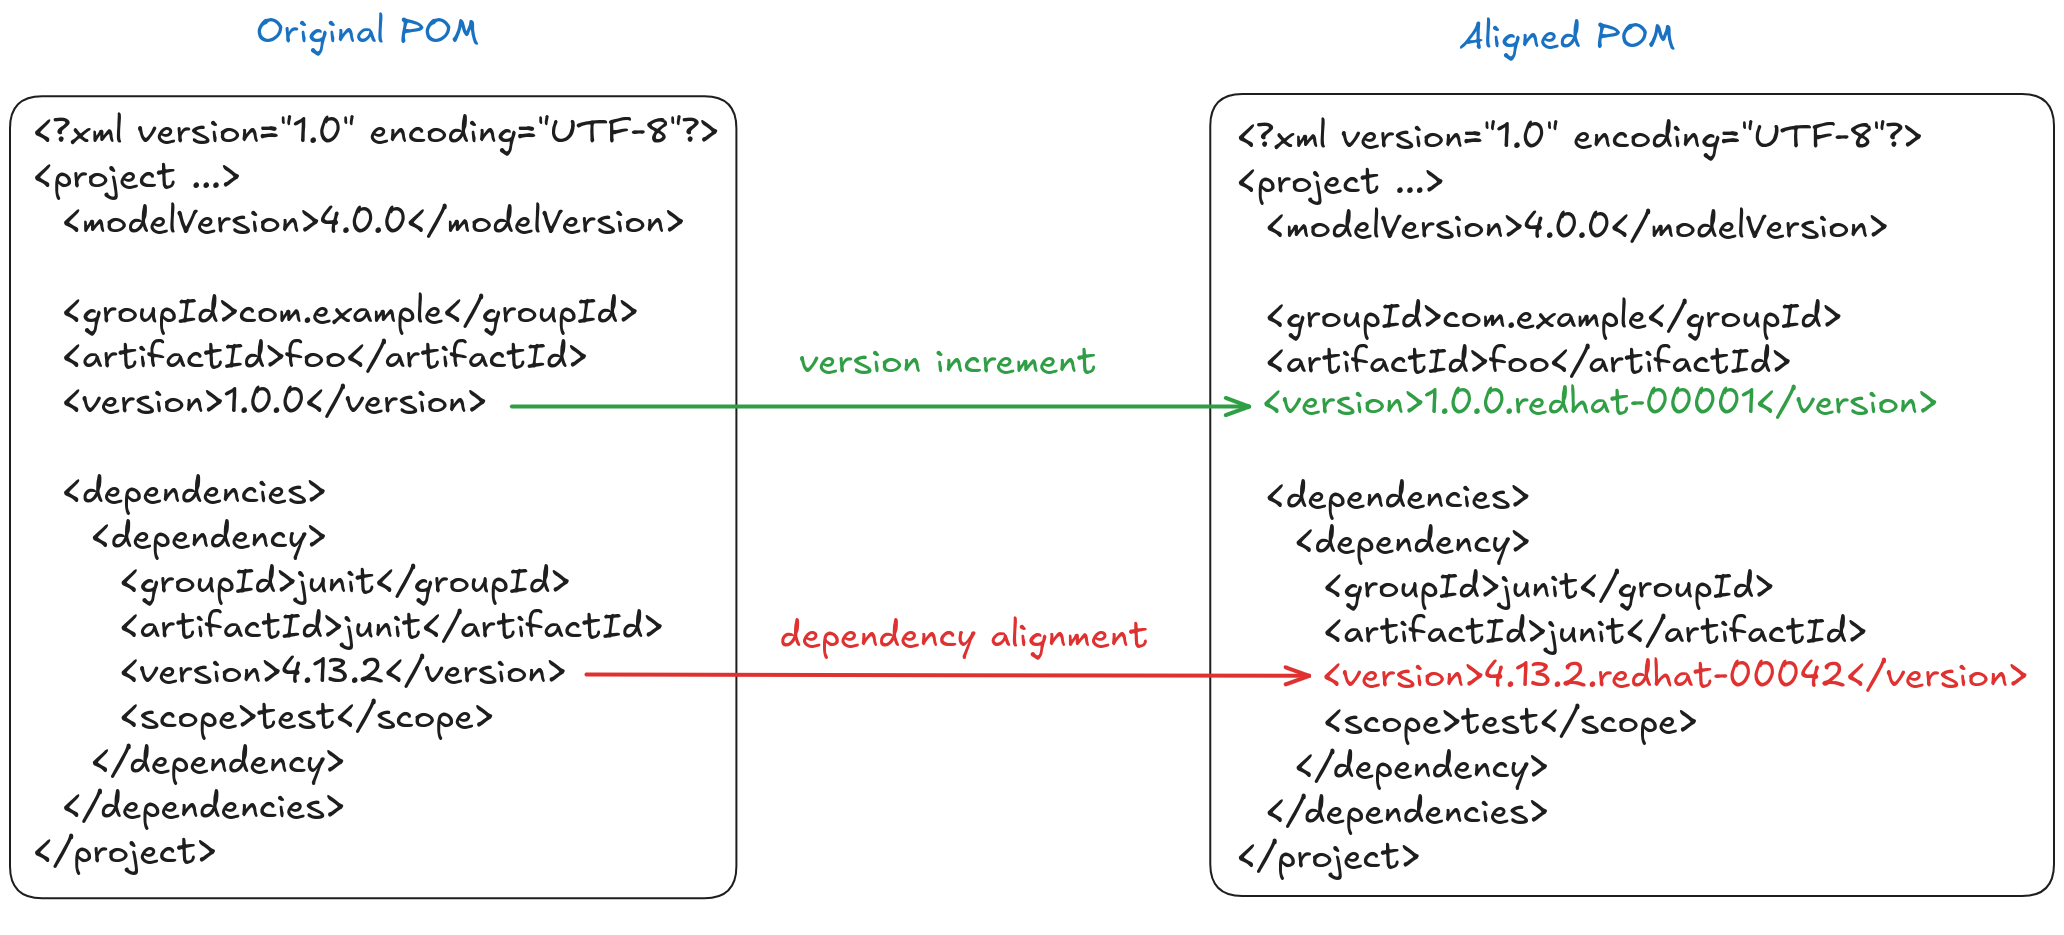
\includegraphics[width=\textwidth]{images/alignment.png}
  \end{center}
  \caption{Example alignment of maven build}
  \label{fig:alignment}
\end{figure}

  \item \textbf{Automatic build scheduling:} Dependencies of build \textit{B} which are used by \textit{B} and need to be (newly) built are built before build \textit{B} is started.

  \item \textbf{Support for multiple build tools:} Provide support for Maven, Gradle, NPM, and SBT builds.

  \item \textbf{Ability to re-use build configurations:} Build configuration of the concrete product version can be re-used in its product milestones.

  \item \textbf{Build cancellation:} Ability to cancel running build.

\end{itemize}

\end{document}
